\documentclass[]{article}

% Imports the catppuccin theme, using the mocha flavor,
% from the directory above. Actual implementation
% wouldn't need the import package unless the theme
% and the document are in different directories.
\usepackage{import}
\usepackage{xcolor}
\usepackage{cancel}
\usepackage{mathtools}

% For permutations and combinations
\newcommand\Myperm[2][^n]{\prescript{#1\mkern-2.5mu}{}P_{#2}}
\newcommand\Mycomb[2]{\prescript{#1\mkern-0.5mu}{}C_{#2}}

% Colors
\definecolor{yorhabg}{HTML}{FFFFFF}
\definecolor{yorhafg}{HTML}{000000}
\definecolor{yorhagrid}{HTML}{B5AF9C}
\definecolor{mred}{HTML}{D67069}
\definecolor{mblue}{HTML}{6887A1}

\pagecolor{yorhabg}
\color{yorhafg}

\usepackage{preamble}

% Removes padding above title
\usepackage{titling}
\setlength{\droptitle}{-10em}

% Font package
\usepackage[T1]{fontenc}

\usepackage{fouriernc}

\usepackage{sectsty}
\usepackage{graphicx}
\usepackage{amsmath}
\usepackage{amsfonts}
\usepackage{amssymb}
\usepackage[skins, most]{tcolorbox}

\DeclareMathOperator{\sgn}{sgn}

\usepackage{tikz}
\usepackage{eso-pic}
\usetikzlibrary{calc,shadows.blur}
\usetikzlibrary{angles, quotes}
\usetikzlibrary{3d}

% Margins
\topmargin=0in
\evensidemargin=0in
\oddsidemargin=0in
\textwidth=6.5in
\textheight=9.0in
\headsep=0.25in

\AtBeginEnvironment{tcolorbox}{\small}

\newtcolorbox{imp}{enhanced,arc=0mm,colback=yorhabg,colframe=mred,leftrule=10mm,coltext=yorhafg,%
overlay={\node[anchor=west,outer sep=2pt] at (frame.west) {
\includegraphics[width=6mm]{images/imageb.png}}; }}

\newtcolorbox{shortcut}{enhanced,arc=0mm,colback=yorhabg,colframe=mred,leftrule=10mm,coltext=yorhafg, coltitle=yorhabg, title=\texttt{Shortcut.}, 
overlay={\node[anchor=west,outer sep=2pt] at (frame.west) {
\includegraphics[width=6mm]{images/imageb.png}}; }}

\newtcolorbox{question}{
    enhanced, 
    colback=yorhabg,
    colframe=mblue,
    coltext=yorhafg,
    coltitle=yorhabg,
    attach boxed title to top left={yshift*=-\tcboxedtitleheight}, 
    title=\texttt{Question.},
    boxed title size=title,
    boxed title style={%
        rounded corners=northeast, 
        rounded corners=northwest, 
        colback=tcbcolframe, 
        boxrule=0pt,
    },
    underlay boxed title={%
        \path[fill=tcbcolframe] (title.south west)--(title.south east) 
            to[out=0, in=180] ([xshift=5mm]title.east)--
            (title.center-|frame.east)
            [rounded corners=5pt] |- 
            (frame.north) -| cycle; 
    },
}

\newcommand\bb[1]{\textcolor{yorhafg}{\textbf{#1}}}

\title{\textbf{CSCA67 - Assignment \#1}}
\author{ Satyajit Datta }
\date{\today}

\begin{document}

\maketitle    

\section*{1. Logical Equivalence}
For each of the following pairs of expressions, either prove that the two expressions are equivalent or prove that
they are not. (Clearly state what you are proving!) Do not use truth tables.
\vspace{1em}
\hrule
\vspace{1em}

\begin{question}
    $(a \rightarrow b) \land (b \rightarrow c)$ and $a \rightarrow c$
\end{question}
\begin{center}
        \text{We are proving that the two expressions are not equivalent.} \\
        \text{Consider the case where } a = \text{True}, b = \text{False}, c = \text{True}. \\
\end{center}
\begin{align*}
    & (a \rightarrow b) \land (b \rightarrow c) & & a \rightarrow c\\
    \equiv\; & (T \rightarrow F) \land (F \rightarrow T) & \equiv\; & T \rightarrow T\\
    \equiv\; & F \land T & \equiv\; & \bb{T}\\
    \equiv\; & \bb{F} && \\
\end{align*}
\begin{center}
    $\therefore$ The two expressions are not equivalent. $\blacksquare$
\end{center}

\begin{question}
    $a \land (a \rightarrow b)$ and $a \rightarrow b$
\end{question}
\begin{center}
    \text{We are proving that the two expressions are not equivalent.} \\
    \text{Consider the case where} a = \text{False}, b = \text{True}
\end{center}
\begin{align*}
    & a \land (a \rightarrow b) &  & a \rightarrow b \\
    \equiv\; & F \land (F \rightarrow T)  & \equiv\; & F \rightarrow T\\
    \equiv\; & F \land T & \equiv\; \bb{T} \\
    \equiv\; & \bb{F}
\end{align*}
\begin{center}
    $\therefore$ The two expressions are not equivalent. $\blacksquare$
\end{center}

\begin{question}
    $(a \rightarrow b) \land (a \rightarrow c)$ and $a \rightarrow (b \land c)$
\end{question}
\begin{center}
    \text{We are proving that the two expressions \bb{are} equivalent.}
\end{center}
\begin{align*}
    & (a \rightarrow b) \land (a \rightarrow c) & & a \rightarrow (b \land c) \\
    \equiv\; & (\neg a \lor b) \land (\neg a \lor c) \quad \text{(Conditional Law)} & \equiv\; & \mathbf{\neg a \lor (b \land c)} \quad \text{(Conditional Law)} \\
    \equiv\; & \mathbf{\neg a \lor (b \land c)} \quad \text{(Distributive Law)} & & \\
\end{align*}
\begin{center}
    $\therefore$ The two expressions are equivalent. $\blacksquare$
\end{center}

\begin{question}
    $(a \rightarrow c) \land (b \rightarrow c)$ and $(a \lor b) \rightarrow c$
\end{question}
\begin{center}
    \text{We are proving that the two expressions \bb{are} equivalent.}
\end{center}
\begin{align*}
    & (a \rightarrow c) \land (b \rightarrow c) & & (a \lor b) \rightarrow c \\
    \equiv\; & (\neg a \lor c) \land (\neg b \lor c) \quad \text{(Conditional Law)} & \equiv\; & \neg(a \lor b) \lor c \quad \text{(Conditional Law)} \\
    \equiv\; & \mathbf{(\neg a \land \neg b) \lor c} \quad \text{(Distributive Law)} & \equiv\; & \mathbf{(\neg a \land \neg b) \lor c} \quad \text{(De Morgan's Theorem)} \\
\end{align*}
\begin{center}
    $\therefore$ The two expressions are equivalent. $\blacksquare$
\end{center}

\begin{question}
    $a \iff b$ and $(a \land b) \lor (\neg a \land \neg b)$
\end{question}
\begin{center}
    \text{We are proving that the two expressions \bb{are} equivalent.}
\end{center}
\begin{align*}
    & a \iff b & & \mathbf{(a \land b) \lor (\neg a \land \neg b)} \\
    \equiv\; & (a \rightarrow b) \land (b \rightarrow a) \quad \text{(Biconditional Law)} \\
    \equiv\; & (\neg a \lor b ) \land (\neg b \lor a) \quad \text{(Conditional Law)} \\
    \equiv\; & (\neg a \land \neg b) \lor (\neg a \land a) \lor (b \land \neg b) \lor (b \land a) \quad \text{(Distributive Law)} \\ 
    \equiv\; & \mathbf{(\neg a \land \neg b) \lor (a \land b)} \quad \text{(Negation Law)}
\end{align*}
\begin{center}
    $\therefore$ The two expressions are equivalent. $\blacksquare$
\end{center}

\begin{question}
    $a \rightarrow (b \rightarrow (c \rightarrow d))$ and $(a \land b \land c) \rightarrow d$
\end{question}
\begin{center}
    \text{We are proving that the two expressions \bb{are} equivalent.}
\end{center}
\begin{align*}
    & a \rightarrow (b \rightarrow (c \rightarrow d)) & & \mathbf{(a \land b \land c) \rightarrow d} \\
    \equiv\; & \neg a \lor (\neg b \lor (\neg c \lor d)) \quad \text{(Conditional Law)} \\
    \equiv\; & (\neg a \lor \neg b \lor \neg c) \lor d \\
    \equiv\; & \neg(a \land b \land c) \lor d \quad \text{(De Morgan's)} \\
    \equiv\; & \mathbf{(a \land b \land c) \rightarrow d} \quad \text{(Conditional Law)} \\
\end{align*}
\begin{center}
    $\therefore$ The two expressions are equivalent. $\blacksquare$
\end{center}

\begin{question}
    $(a \rightarrow b) \lor (b \rightarrow a)$ and $a \iff b$
\end{question}
\begin{center}
        \text{We are proving that the two expressions are not equivalent.} \\
        \text{Consider the case where } a = \text{True}, b = \text{False}. \\
\end{center}
\begin{align*}
    & (a \rightarrow b) \lor (b \rightarrow a) & & a \iff b\\
    \equiv\; & (T \rightarrow F) \lor (F \rightarrow T) & \equiv\; & (a \rightarrow b) \land (b \rightarrow a) \quad \text{(Biconditional Law)}\\
    \equiv\; & F \lor T & \equiv\; &  (T \rightarrow F) \land (F \rightarrow T)\\
    \equiv\; & \mathbf{T} & \equiv\; & F \land T \\
    & &  \equiv\; & \mathbf{F} \\
\end{align*}
\begin{center}
    $\therefore$ The two expressions are not equivalent. $\blacksquare$
\end{center}

\begin{question}
    $a \iff b$ and $\neg a \iff \neg b$
\end{question}
\begin{center}
    \text{We are proving that the two expressions \bb{are} equivalent.}
\end{center}
\begin{align*}
    & a \iff b & & \neg a \iff \neg b \\
    \equiv\; & (a \rightarrow b) \land (b \rightarrow a) \quad \text{(Biconditional Law)} & \equiv & (\neg a \rightarrow \neg b) \land (\neg b \rightarrow \neg a) \quad \text{(Biconditional Law)}\\
    \equiv\; & (\neg a \lor b) \land (\neg b \lor a) \quad \text{(Conditional Law)} & \equiv & (\neg\neg a \lor \neg b) \land (\neg\neg b \lor \neg a) \quad \text{(Conditional Law)}\\
    & & \equiv & (a \lor \neg b) \land (b \lor \neg a) \quad \text{(Double Negation law)} \\
\end{align*}
\begin{center}
    $\therefore$ The two expressions are equivalent. $\blacksquare$
\end{center}

\begin{question}
    $(a \land b) \rightarrow (c \land d)$ and $((a \rightarrow c) \land (a \rightarrow d)) \land ((b \rightarrow c) \land (b \rightarrow d))$
\end{question}
\begin{center}
        \text{We are proving that the two expressions are not equivalent.} \\
        \text{Consider the case where } a = \text{True}, b = \text{False}, c = \text{False}, d = \text{False}.\\
\end{center}
\begin{align*}
    & (a \land b) \rightarrow (c \land d) & & ((a \rightarrow c) \land (a \rightarrow d)) \land ((b \rightarrow c) \land (b \rightarrow d))\\
    \equiv\; & (T \land F) \rightarrow (F \land F) & \equiv\; & ((T \rightarrow F) \land (T \rightarrow F)) \land ((F \rightarrow F) \land (F \rightarrow F)) \\
    \equiv\; & F \lor T & \equiv\; &  (F \land F) \land (T \land T)\\
    \equiv\; & \mathbf{T} & \equiv\; & F \land F \\
    & &  \equiv\; & \mathbf{F} \\
\end{align*}
\begin{center}
    $\therefore$ The two expressions are not equivalent. $\blacksquare$
\end{center}

\begin{question}
        $(a \lor b) \rightarrow (c \land d)$ and $((a \rightarrow c) \land (a \rightarrow d)) \land ((b \rightarrow c) \land (b \rightarrow d))$
\end{question}
\begin{center}
        \text{We are proving that the two expressions are equivalent.} \\
\end{center}
\begin{align*}
    & (a \lor b) \rightarrow (c \land d) & & ((a \rightarrow c) \land (a \rightarrow d)) \land ((b \rightarrow c) \land (b \rightarrow d))\\
    \equiv\; & \neg(a \lor b) \lor (c \land d) \quad \text{(Conditional Law)} \quad \vrule & \equiv\; & ((\neg a \lor c) \land (\neg a \lor d)) \land ((\neg b\lor c) \land (\neg b \lor d)) \quad \text{(Conditional Law)}\\
    & \quad \vrule & \equiv\; &  (\neg a \lor (c \land d))\land (\neg b \lor (c \land d)) \quad \text{(Distributive Law)}\\
    & \quad \vrule & \equiv\; & (\neg a \land \neg b ) \lor (c \land d) \quad \text{(Distributive Law)} \\
    & \quad \vrule &  \equiv\; & \neg(a \lor b) \lor (c \land d) \quad \text{(De Morgan's law)} \\
\end{align*}
\begin{center}
    $\therefore$ The two expressions are equivalent. $\blacksquare$
\end{center}

\section*{2. Logical Equivalence}
Determine whether each statement below is a tautology, a contradiction, or neither. Prove your result. Do not
use truth tables.

\begin{center}
    Note that for this section, I will refer to tautologies with $\top$ and contradictions with $\bot$.
\end{center}
\vspace{0.1in}
\hrule
\vspace{0.1in}
\begin{question}
    $(a \rightarrow b) \lor (b\ \rightarrow a)$
\end{question}
\begin{align*}
    & (a \rightarrow b) \lor (b \rightarrow a) \\
    \equiv\; & (\neg a \lor b) \lor (\neg b \lor a) \quad \text{(Conditional Law)} \\
    \equiv\; & (\neg a \lor a) \lor (\neg b \lor b) \quad \\
    \equiv\;&  \top \lor \top \quad \text{(Tautology Law)} \\
    \equiv\; & \top \quad \text{(Tautology Law)}
\end{align*}
\begin{center}
    $\therefore$ The statement is a tautology. $\blacksquare$
\end{center}

\begin{question}
    $(((a \rightarrow b) \land (b \rightarrow c)) \land a) \land \neg c$
\end{question}
\begin{align*}
    & (((a \rightarrow b) \land (b \rightarrow c)) \land a) \land \neg c \\
    \equiv\; & (((\neg a \lor b) \land (\neg b \lor c)) \land a) \land \neg c \quad \text{(Conditional Law)} \\
    \equiv\; & ((\neg a \land a) \lor (a\land b) \land (\neg b \lor c)) \land \neg c \quad \text{(Distributive Law)} \\
    \equiv\; & (\bot \lor (a\land b) \land (\neg b \lor c)) \land \neg c \quad \text{(Contradiction Law)} \\
    \equiv\; & ((a\land b) \land (\neg b \lor c)) \land \neg c \quad \text{(Contradiction Law)} \\
    \equiv\; & ((a \land \neg b \land b) \lor (a \land b \land c)) \land \neg c \quad \text{(Distributive Law)} \\
    \equiv\; & ((a \land \bot) \lor (a\land b\land c)) \land \neg c \quad \text{(Contradiction Law)} \\
    \equiv\; & (\bot \lor (a\land b\land c)) \land \neg c \quad \text{(Contradiction Law)} \\
    \equiv\; & (a\land b\land c) \land \neg c \quad \text{(Contradiction Law)} \\
    \equiv & a \land b \land c \land \neg c \quad \\
    \equiv\; & a \land b \land \bot \quad \text{(Contradiction Law)} \\
    \equiv\; & \bot \quad \text{(Contradiction Law)}
\end{align*}
\begin{center}
    $\therefore$ The statement is a contradiction. $\blacksquare$
\end{center}
\vspace{1.7in}
\begin{question}
    $(((a \rightarrow b) \land (b \rightarrow c)) \land a) \land  c$
\end{question}
\begin{align*}
    & (((a \rightarrow b) \land (b \rightarrow c)) \land a) \land c \\
    \equiv\; & (((\neg a \lor b) \land (\neg b \lor c)) \land a) \land c \quad \text{(Conditional Law)} \\
    \equiv\; & ((\neg a \land a) \lor (a\land b) \land (\neg b \lor c)) \land c \quad \text{(Distributive Law)} \\
    \equiv\; & (\bot \lor (a\land b) \land (\neg b \lor c)) \land c \quad \text{(Contradiction Law)} \\
    \equiv\; & ((a\land b) \land (\neg b \lor c)) \land c \quad \text{(Contradiction Law)} \\
    \equiv\; & ((a \land \neg b \land b) \lor (a \land b \land c)) \land  c \quad \text{(Distributive Law)} \\
    \equiv\; & ((a \land \bot) \lor (a\land b\land c)) \land  c \quad \text{(Contradiction Law)} \\
    \equiv\; & (\bot \lor (a\land b\land c)) \land c \quad \text{(Contradiction Law)} \\
    \equiv\; & (a\land b\land c) \land c \quad \text{(Contradiction Law)} \\
    \equiv\; & a \land b \land c \land c \quad \\
    \equiv\; & a \land b \land c \quad \text{(Idempotent Law)}
\end{align*}
\begin{center}
    $\therefore$ The statement is a neither a tautology nor a contradiction. $\blacksquare$
\end{center}

\begin{question}
    $a \rightarrow \neg a$
\end{question}
\begin{align*}
    & a \rightarrow \neg a \\
    \equiv\; & \neg a \lor \neg a \quad \text{(Conditional Law)} \\
    \equiv\; & \neg a \quad \text{(Idempotent Law)} \\
\end{align*}
\begin{center}
    $\therefore$ Therefore, the statement is neither a tautology nor a contradiction. $\blacksquare$
\end{center}

\begin{question}
    $(a \land (a \rightarrow b)) \rightarrow b$
\end{question}
\begin{align*}
    \equiv\; & (a \land (a \rightarrow b)) \rightarrow b \\
    \equiv\; & \neg(a \land (a \rightarrow b)) \lor b \quad \text{(Conditional Law)} \\
    \equiv\; & \neg(a \land (\neg a \lor b)) \lor b \quad \text{(Conditional Law)} \\
    \equiv\; & \neg((a \land \neg a) \lor (a \land b)) \lor b \quad \text{(Distributive Law)} \\
    \equiv\; & \neg(\bot \lor (a\land b)) \lor b \quad \text{(Contradiction Law)}\\
    \equiv\; &  \neg(a \land b) \lor b \quad \text{(Contradiction Law)} \\
    \equiv\; & \neg a \lor \neg b \lor b \quad \text{(De Morgan's Law)} \\
    \equiv\; & \neg a \lor \top \quad \text{(Tautology Law)} \\
    \equiv\; & \top \quad \text{(Tautology Law)}
\end{align*}
\begin{center}
    $\therefore$ The statement is a tautology. $\blacksquare$
\end{center}
\section*{3. Deductive Reasoning}
For each of the following arguments:

\quad • If the argument is valid, you need to both:

\quad \quad 1. Prove the argument is valid by using a truth table. The truth table must be in the format we used in class, and the variables must appear in alphabetical order.

\quad \quad 2. Prove the argument is valid by using Rules of Inference.



\quad • If the argument is not valid, provide an assignment of truth values to variables and demonstrate that it proves
that the argument is not valid.
\vspace{0.1in}
\hrule
\vspace{0.1in}

\begin{question}
    If the weather is good, I either go running or swimming. I don’t go running and swimming at the same time.
Therefore, if the weather is good and I go running, then I do not go swimming. Also, if the weather is good and
I go swimming, then I do not go running.
\end{question}
\[
    \text{Statements} = \begin{cases}
        W = \text{The weather is good.} \\
        R = \text{I go running.} \\
        S = \text{I go swimming.}
    \end{cases} \\
\]
    
\begin{center}
    \text{Thus, our our premises and conclusions are:}
\end{center}    
\begin{align*}
    W \rightarrow (R \lor S) & \quad (1) \\
    \neg(R \land S) & \quad (2) \\
    \overline{((W \land R) \rightarrow \neg S) \land ((W \land S) \rightarrow \neg R)} &  \quad \text{Conclusion}
\end{align*}

\begin{figure}[h!]
    \begin{center}
        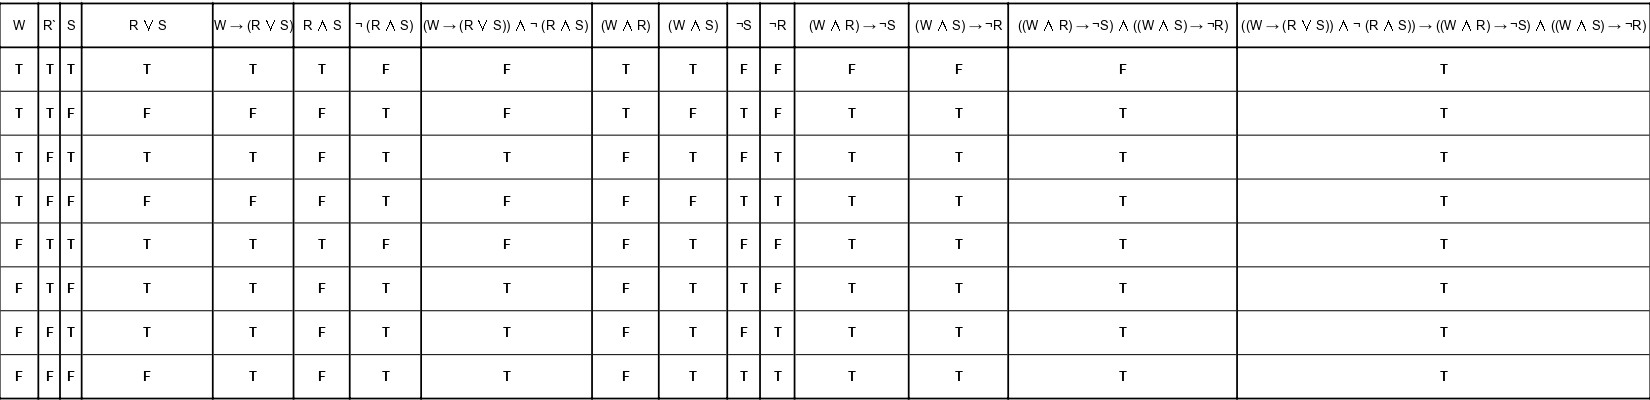
\includegraphics[totalheight=4cm]{images/Q3P1.jpg}
        
    \end{center}
    \caption{Since (1) $\land$ (2) $\to$ Conclusion is is a tautology, the argument is valid. $\blacksquare$}
    \caption{Truth Table for Question 3.1}
\end{figure}

\begin{center}
    \text{Since the conclusion is true in all cases where the premises are true, the argument is valid.} \\
    \text{Now, we will prove the argument is valid using Rules of Inference.}\\
    \text{Some new statements we can create are:}
\end{center}
\begin{align*}
    \neg W \lor R \lor S \quad & \text{(1), Conditional Law} \hfill & \text{(3)} \\
    \neg R \lor \neg S \quad & \text{(2), De Morgan's Theorem} \hfill & \text{(4)} \\
    \neg S \lor S \lor \neg W \quad & \text{(3), (4), Resolution} \hfill & \text{(5)} \\
    \neg W \lor \neg S \lor \neg R \quad & \text{(4), (5), Resolution} \hfill & \text{(6)} \\
    \neg (W \land R) \lor \neg S \quad & \text{(6), De Morgan's Theorem} \hfill & \text{(7)} \\
    \neg (W \land S) \lor \neg R \quad & \text{(6), De Morgan's Theorem} \hfill & \text{(8)} \\
    (W \land R) \rightarrow \neg S \quad & \text{(7), Conditional Law} \hfill & \text{(9)} \\
    (W \land S) \rightarrow \neg R \quad & \text{(8), Conditional Law} \hfill & \text{(10)} \\
    ((W \land R) \rightarrow \neg S) \land ((W \land S) \rightarrow \neg R) \quad & \text{(9), (10), Conjunction} \hfill & \text{(11)} \\
\end{align*}
\begin{center}
    $\therefore$ Since (11) = Conclusion, The argument is valid. $\blacksquare$
\end{center}

\begin{question}
    To get a good grade in CSCA67, it is necessary for me to attend lectures and do the assigned readings. I attend
lectures and I do the assigned readings. Therefore, I will get a good grade in CSCA67.
\end{question}
\[
    \text{Statements} = \begin{cases}
        G = \text{I get a good grade in CSCA67.} \\         
        L = \text{I attend lectures.} \\
        R = \text{I do the assigned readings.}
    \end{cases} \\
\]
    
\begin{center}
    \text{Thus, our our premises and conclusions are:}
\end{center}    
\begin{align*}
    G \rightarrow (L \land R) & \quad (1) \\
    \underline{L \land R} & \quad (2) \\
    G &  \quad \text{Conclusion}
\end{align*}
\begin{center}
    \text{This argument is not valid. Consider the case where }  \\
    G = \text{False}, L = \text{True}, R = \text{True} \\
    \text{Note that L and R must be true, due to premise (2). Therefore the only variable we assigned a value to is G.} \\
\end{center}
\begin{align*}
    & \underline{\text{Premise (1)}} & & \underline{\text{Premise (2)}} & & \underline{\text{Conclusion}} \\
    & G \rightarrow (L \land R) & & L \land R & & G \\
    \equiv\; & F \rightarrow (T \land T) & \equiv\; & T & \equiv\; & F \\
    \equiv\; & T & & & & \\
\end{align*}
\begin{center}
    $\therefore$ The argument is not valid, as the premises are true while the conclusion is false. $\blacksquare$
\end{center}

\begin{question}
    To get a good grade in CSCA67, it is sufficient for me to attend lectures and do the assigned readings and solve
all assigned exercises or to already know all course material perfectly from before. I attend lectures and I do
the assigned readings. I solve all assigned exercises. Therefore, I will get a good grade in CSCA67.
\end{question}

\[
    \text{Statements} = \begin{cases}
        G = \text{I get a good grade in CSCA67.} \\         
        L = \text{I attend lectures.} \\
        E = \text{I solve all assigned exercises.} \\
        K = \text{I already know all course material perfectly from before.} \\
        R = \text{I do the assigned readings.} \\
    \end{cases}
\]
\begin{center}
    \text{Thus, our our premises and conclusions are:}
\end{center}
\begin{align*}
    ((L \land R \land E) \lor K) \rightarrow G & \quad (1) \\
    L \land R & \quad (2) \\
    E & \quad (3) \\
    \overline{G} &  \quad \text{Conclusion}
\end{align*}
\begin{figure}[h!]
    \begin{center}
        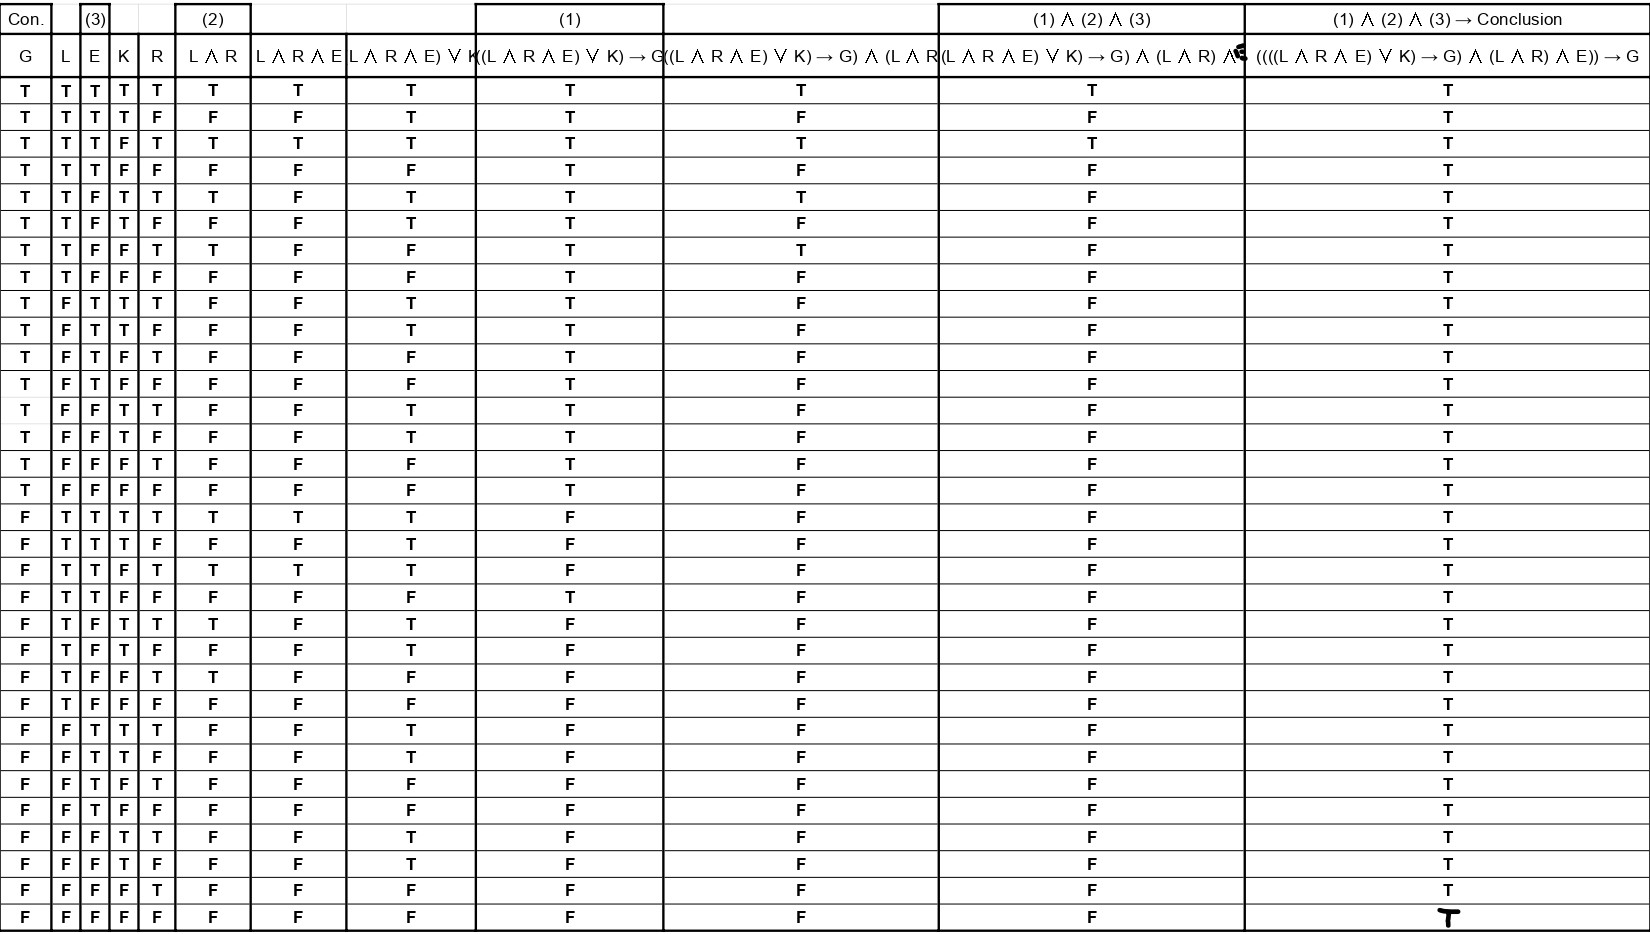
\includegraphics[totalheight=8cm]{images/Q3P3.jpg}
        
    \end{center}
    \caption{Since (1) $\land$ (2) $\land$ (3) $\to$ Conclusion is is a tautology, the argument is valid. $\blacksquare$}
    \caption{Truth Table for Question 3.3}
\end{figure}
\begin{center}
    \text{Since the conclusion is true in all cases where the premises are true, the argument is valid.} \\
    \text{Now, we will prove the argument is valid using Rules of Inference.}\\
    \text{Some new statements we can create are:}
\end{center}
\begin{align*}
    L \land R \land E \quad & \text{(2), (3), Conjunction} \hfill & \text{(4)} \\
    (L \land R \land E) \lor K \quad & \text{(4), Addition} \hfill & \text{(5)} \\
    G \quad & \text{(1), (5), Modus Ponens} \hfill & \text{(6)} \\
\end{align*}
\begin{center}
    $\therefore$ Since (6) = Conclusion, The argument is valid. $\blacksquare$
\end{center}

\begin{question}
    If the butler was in the living room, then he couldn’t have committed the murder. Or, if the cook was in the
kitchen, then she must be innocent. Either the butler is guilty or the cook is guilty. Therefore, either the butler
was not in the living room, or the cook was not in the kitchen.
\end{question}
\[  
    \text{Statements} = 
    \begin{cases}
        B = \text{The butler is guilty.} \\
        C = \text{The cook is guilty.} \\
        L = \text{The butler was in the living room.} \\
        K = \text{The cook was in the kitchen.}
    \end{cases}
\]
\begin{center}
    Thus, our premises and conclusions are:
\end{center}

\begin{align*}
    (L \rightarrow \neg B) \lor (K \rightarrow \neg C) & \quad (1) \\
    B \lor C & \quad (2) \\
    \overline{\neg L \lor \neg K} & \quad \text{Conclusion}
\end{align*}

\begin{center}
    \text{This argument is not valid. Consider the case where }  \\
    B = \text{True}, C = \text{False}, K = \text{True}, L = \text{True} \\
\end{center}
\begin{align*}
    & \underline{\text{Premise (1)}} & & \underline{\text{Premise (2)}} & & \underline{\text{Conclusion}} \\
    & (L \rightarrow \neg B) \lor (K \rightarrow \neg C) & & B \lor C & & \neg L \lor \neg K \\
    \equiv\; & (T \rightarrow F) \lor (T \rightarrow T) & \equiv\; & T \lor F & \equiv\; & \neg T \lor \neg T \\
    \equiv\; & F \lor T & \equiv\; &  T & \equiv\; & F \\
    \equiv\; & T & & & & \\
\end{align*}
\begin{center}
    $\therefore$ The argument is not valid, as the premises are true while the conclusion is false. $\blacksquare$
\end{center}
\begin{question}
    If the butler was in the living room, then he couldn’t have committed the murder. Also, if the cook was in the
kitchen, then she must be innocent. Either the butler is guilty or the cook is guilty. Therefore, either the butler
was not in the living room, or the cook was not in the kitchen.
\end{question}

\[  
    \text{Statements} = 
    \begin{cases}
        B = \text{The butler is guilty.} \\
        C = \text{The cook is guilty.} \\
        L = \text{The butler was in the living room.} \\
        K = \text{The cook was in the kitchen.}
    \end{cases}
\]
\begin{center}
    Thus, our premises and conclusions are:
\end{center}

\begin{align*}
    L \rightarrow \neg B & \quad (1) \\
    K \rightarrow \neg C & \quad (2) \\
    B \lor C & \quad (3) \\
    \overline{\neg L \lor \neg K} & \quad \text{Conclusion}
\end{align*}


\begin{figure}[h!]
    \begin{center}
        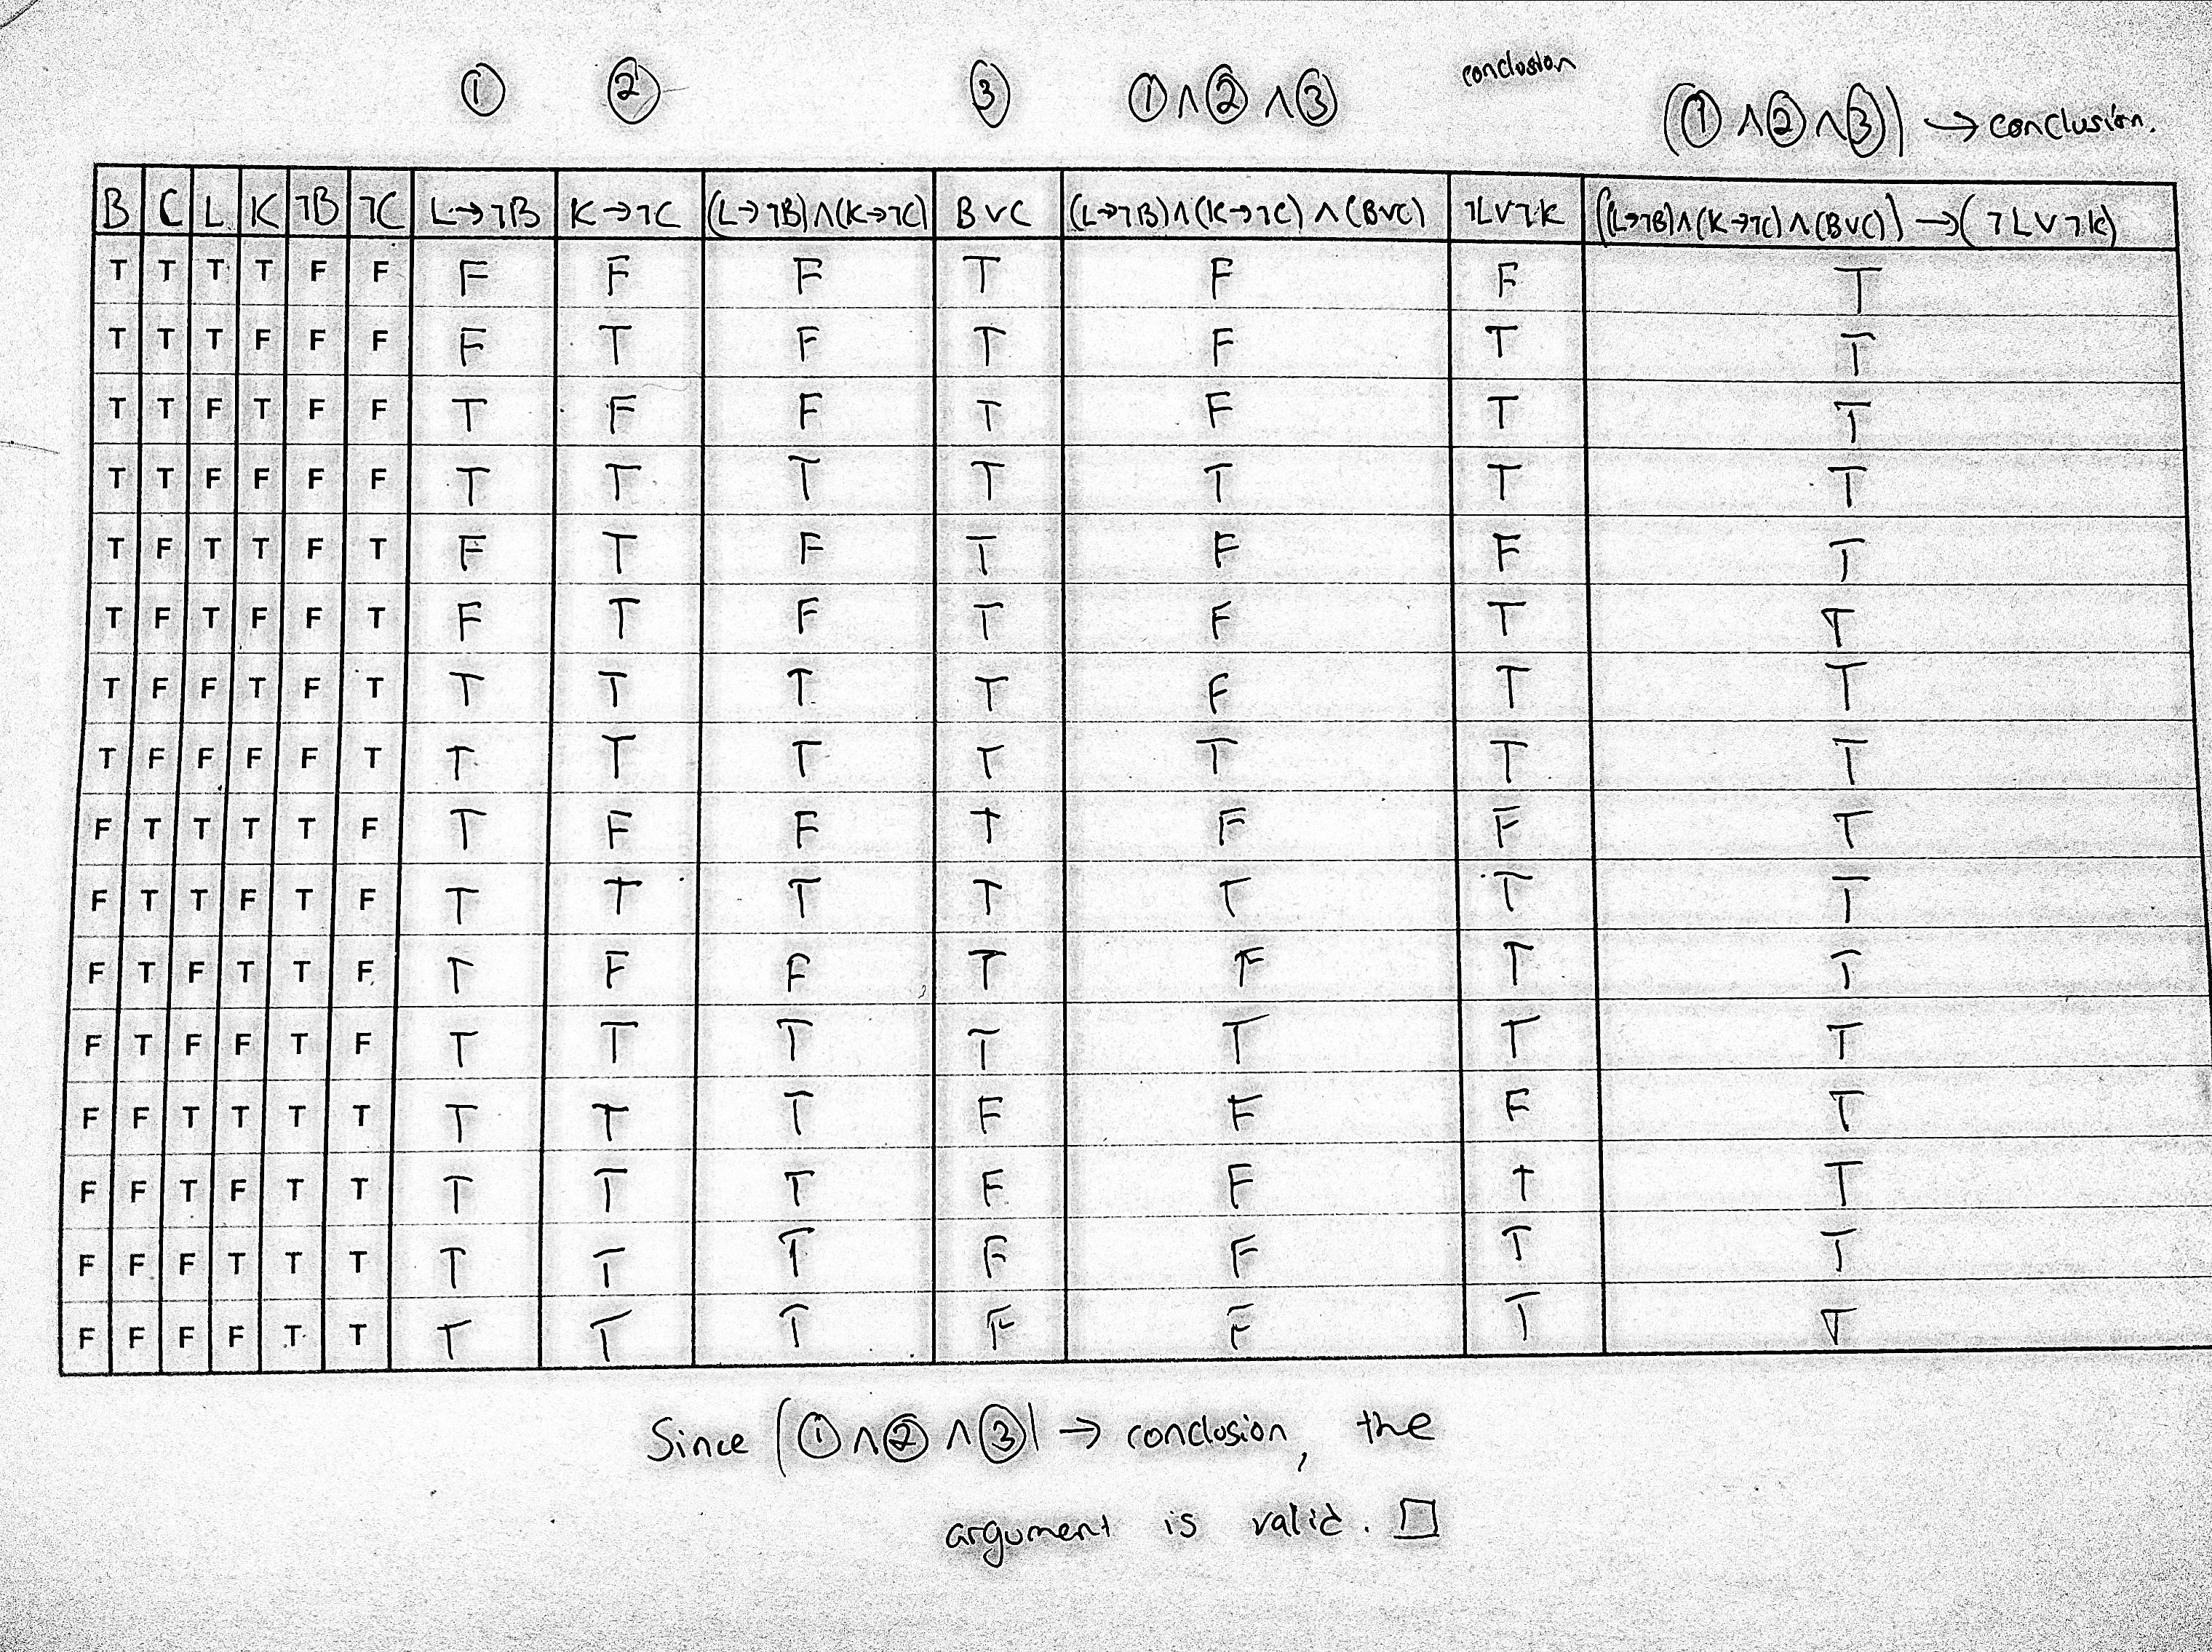
\includegraphics[totalheight=10cm]{images/Q3P5.jpg}
        
    \end{center}
    \caption{Truth Table for Question 3.5}
\end{figure}


\begin{center}
    \text{Since the conclusion is true in all cases where the premises are true, the argument is valid.} \\
    \text{Now, we will prove the argument is valid using Rules of Inference.}\\
    \text{Some new statements we can create are:}
\end{center}
\begin{align*}
    \neg K \lor \neg C \quad & \text{(2), Conditional Law} \hfill & \text{(4)} \\
    \neg K \lor B \quad & \text{(4), (3) Resolution} \hfill & \text{(5)} \\
    \neg L \lor \neg B \quad & \text{(1) Conditional Law} \hfill & \text{(6)} \\
    \neg L \lor \neg K \quad & \text{(6), (5) Resolution} \hfill & \text{(7)} \\
\end{align*}
\begin{center}
    $\therefore$ Since (7) = Conclusion, The argument is valid. $\blacksquare$
\end{center}
\end{document}

